% Show distributions for loose cuts, 5e19 data/MC comparison
% Aggressive cuts, 6.6e20 Projection
% Current efficiency and purity plots as a function of energy

\section{Electron-Like Event Distributions}
The reconstructed energy spectrum of the selected events after the application of the background-rejection cuts is shown in Figure \ref{fig:spectrum_after}. It corresponds to the sum of the reconstructed energies of the shower-like objects, as described in Section \ref{sec:showerenergy}, and the reconstructed energies of the track-like objects, as described in Section \ref{sec:protonenergy}. 

\begin{figure}[htbp]
\centering
  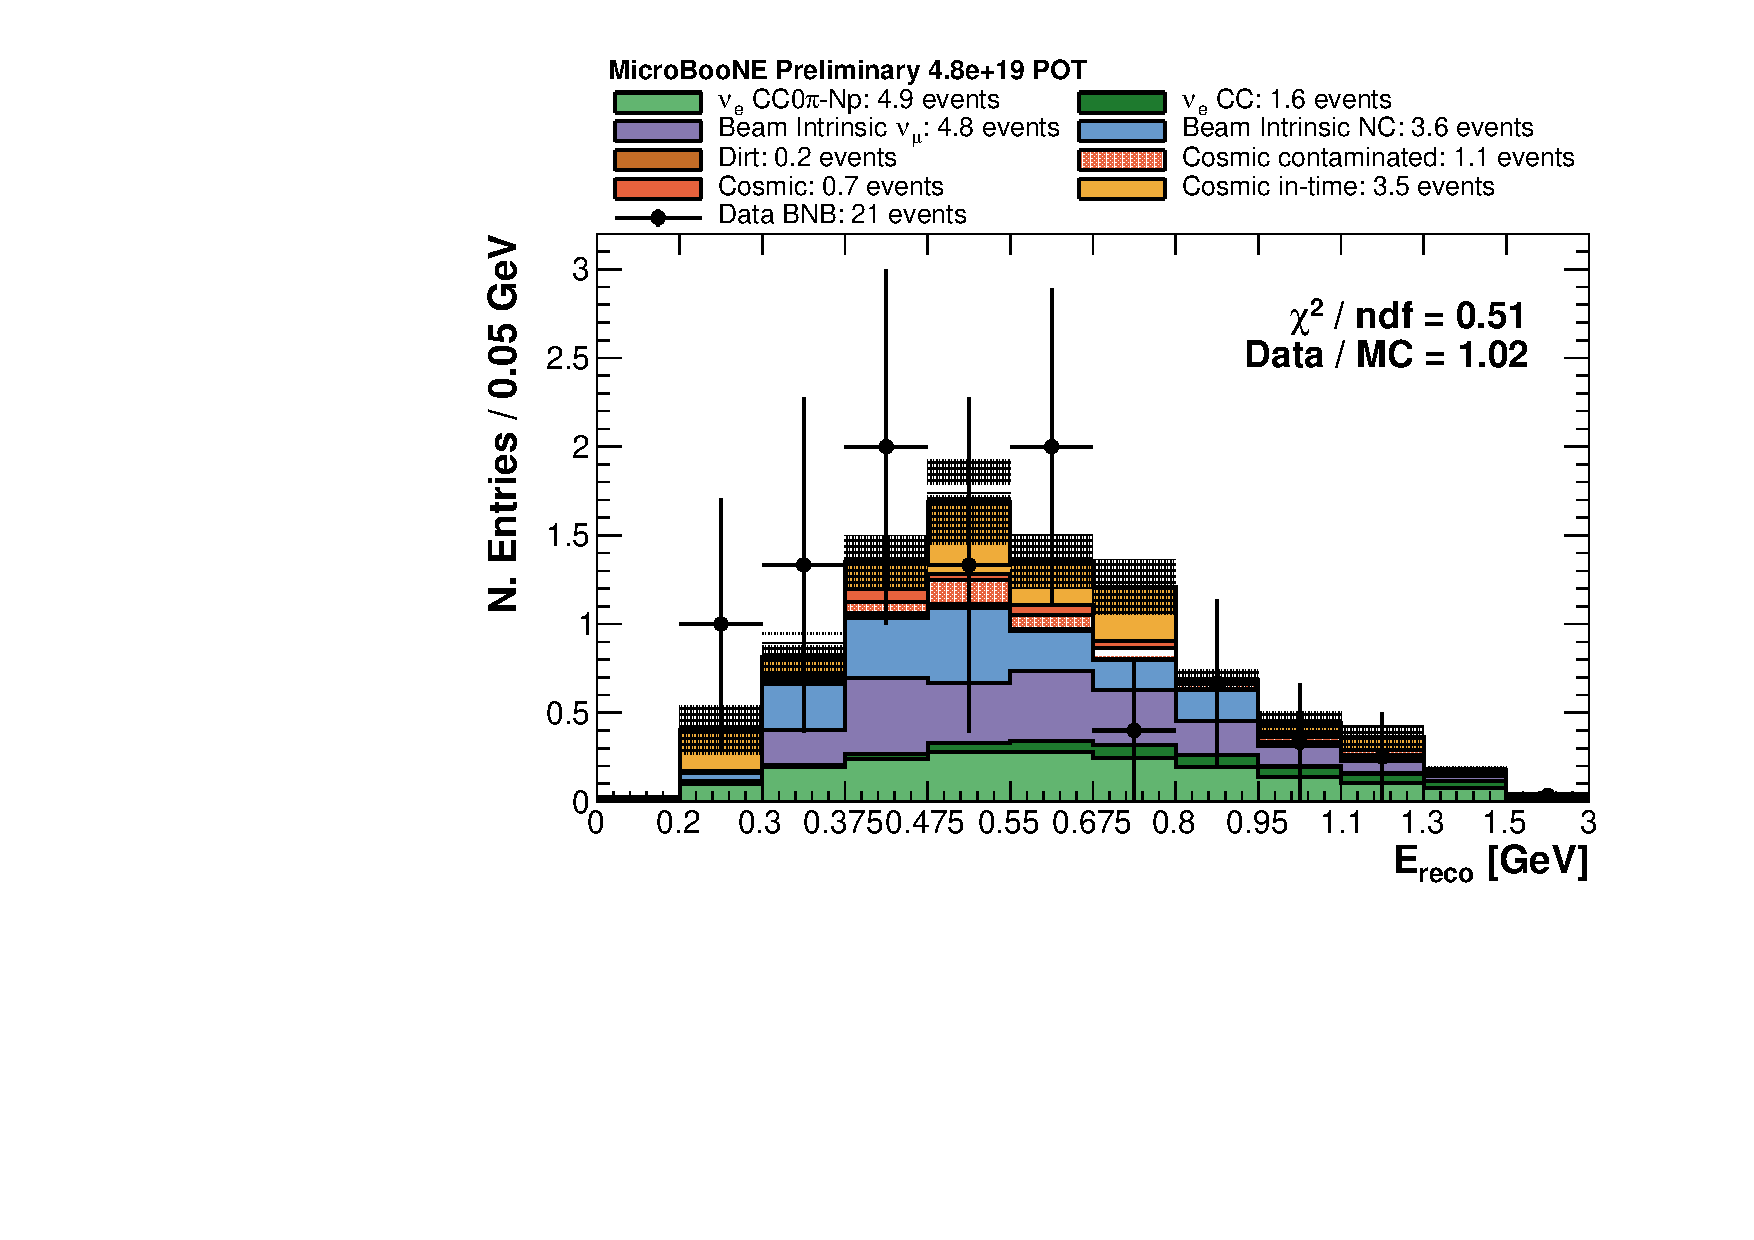
\includegraphics[width=0.65\linewidth]{figures/h_fixed_energy_after.pdf}
    \caption{Reconstructed energy spectrum of the selected events after the background-rejection cuts.}\label{fig:spectrum_after}

\end{figure}


The final number of selected data events in the un-blind \num{4.84e19} POT data sample is 23. These events have been hand-scanned: Figure \ref{fig:evds} shows the event displays of two $\nu_{e}$-like selected data events.


\begin{figure}[htbp]
\centering
  \begin{subfigure}{0.7\textwidth}
  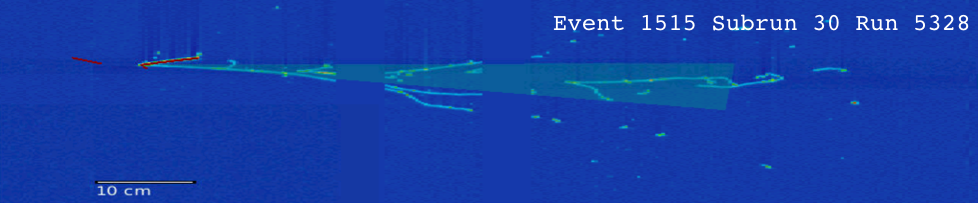
\includegraphics[width=\linewidth]{figures/data1.png}
    \caption{Event 1515, Subrun 30, Run 5328}
\end{subfigure}
  \begin{subfigure}{0.7\textwidth}	
  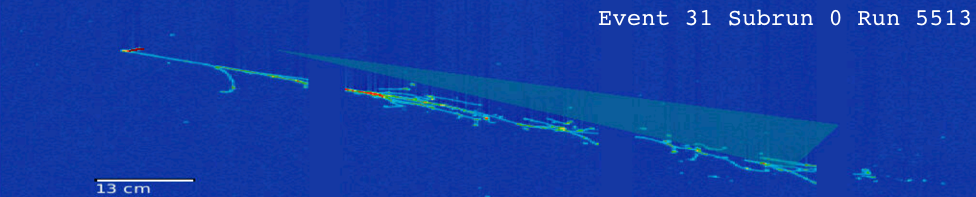
\includegraphics[width=\linewidth]{figures/data2.png}
  \caption{Event 31, Subrun 0, Run 5513}
\end{subfigure}

  \caption{Event displays of the collection plane of two $\nu_{e}$-like data events present in our sample after the background-rejection cuts. The gaps are caused by the presence of missing or unresponsive wires. The red lines correspond to reconstructed track-like objects and the green cones correspond to reconstructed shower-like objects. }
  \label{fig:evds}
\end{figure}

The data BNB distribution is in good agreement with the stacked Monte Carlo + EXT distributions, both in normalization (the integral ratio is 1.03) and in shape ($\chi^2 /\mathrm{n.d.f.} = 0.68$). The signal component ($\nu_{e}$ CC0$\pi$-Np events) represents now the largest component among the event categories with 4.1 events. 

\subsection{Efficiency and purity}
It is now possible to measure the efficiency and the purity of our $\nu_{e}$ CC0$\pi$-Np selection after the background-rejection cuts, as defined in Section \ref{sec:eff}. The background-rejection cuts were aimed to improve the significance of the $\nu_{e}$ CC0$\pi$-Np events in our sample. Thus, the efficiency decreases, from 32.5\% to 11.9\%, since the cuts will eventually remove also some signal events, but the purity increases by a factor of $\sim30$, from 0.5\% to 18.2\%. Figure \ref{fig:effafter} shows the efficiency as a function of the true neutrino energy and the purity as a function of the reconstructed energy, before and after the background rejection cuts. 

\begin{figure}
  \begin{subfigure}{0.48\textwidth}
    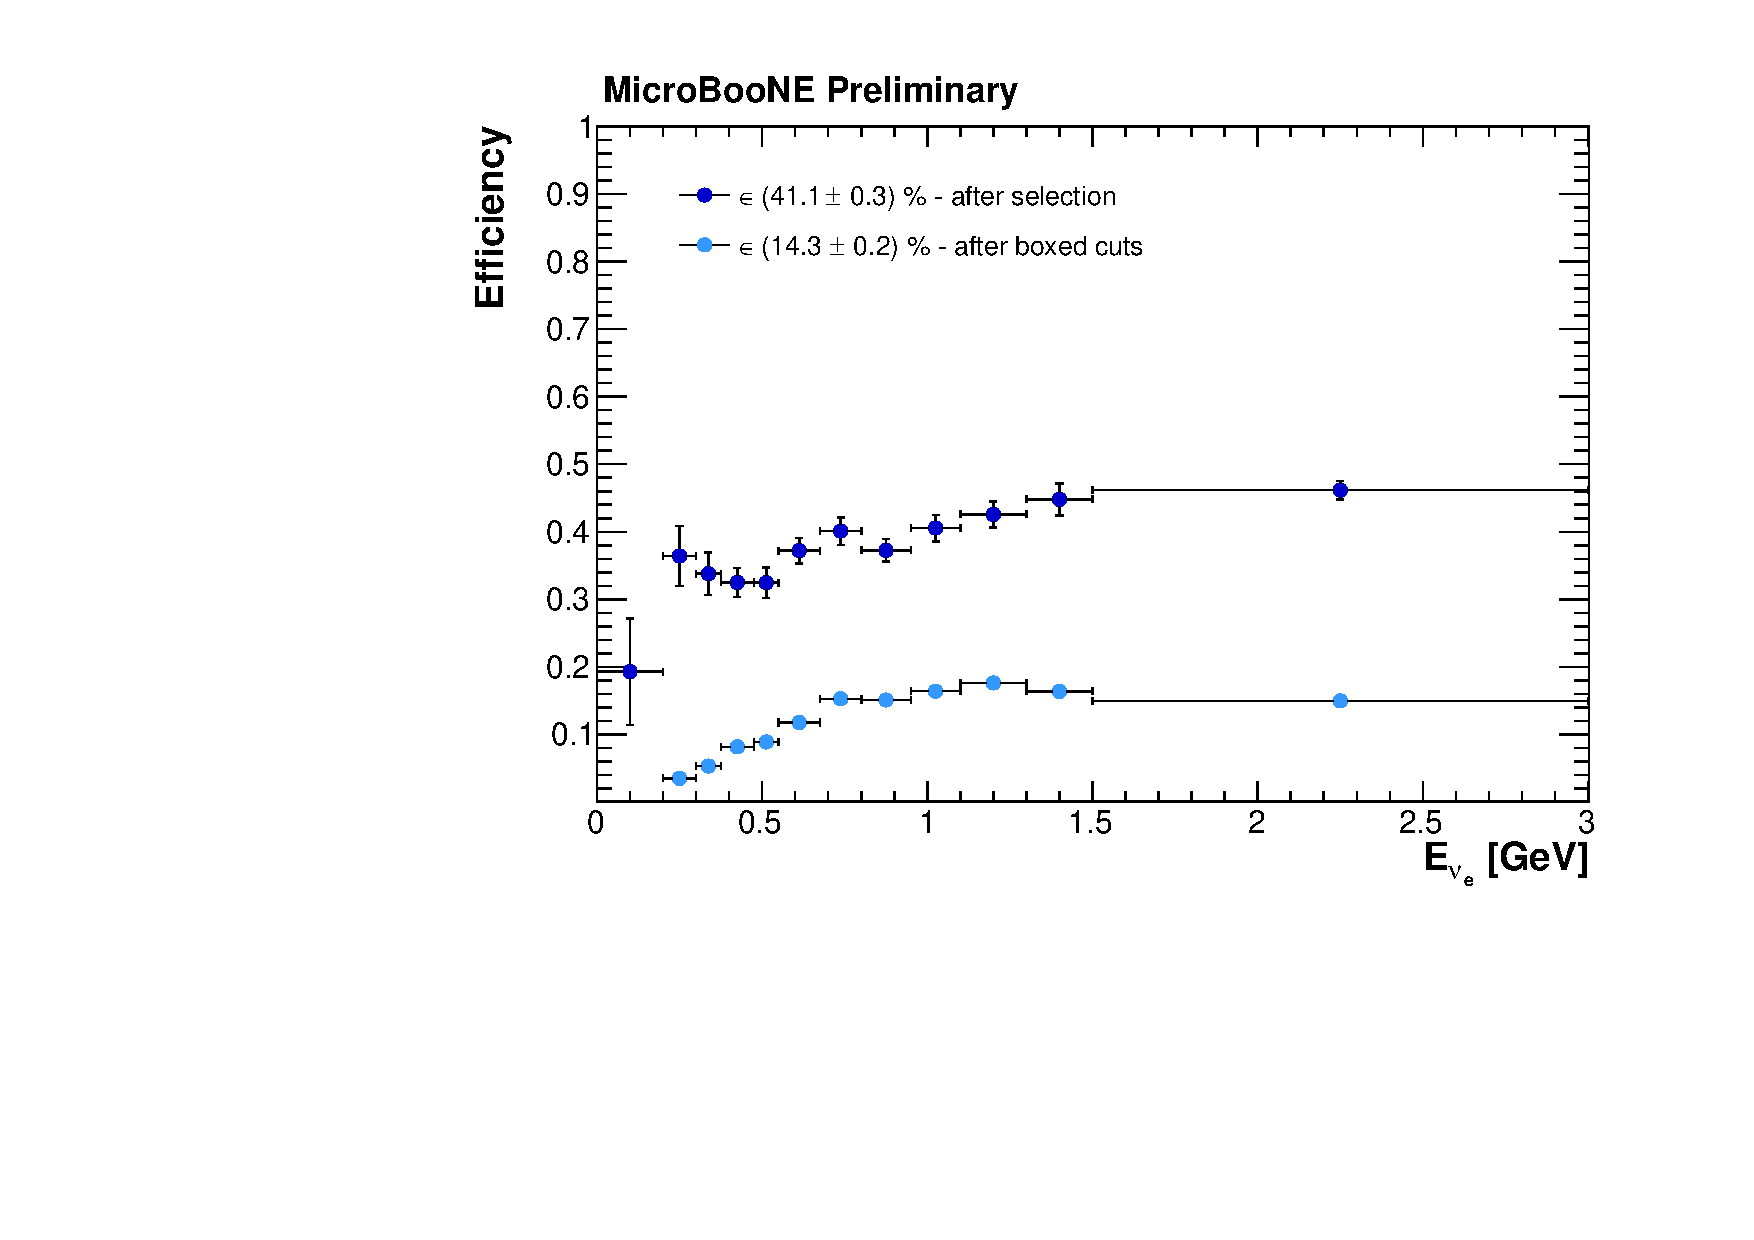
\includegraphics[width=\linewidth]{figures/eff_after.pdf}
    \caption{Efficiency} 
  \end{subfigure}
    \begin{subfigure}{0.48\textwidth}
    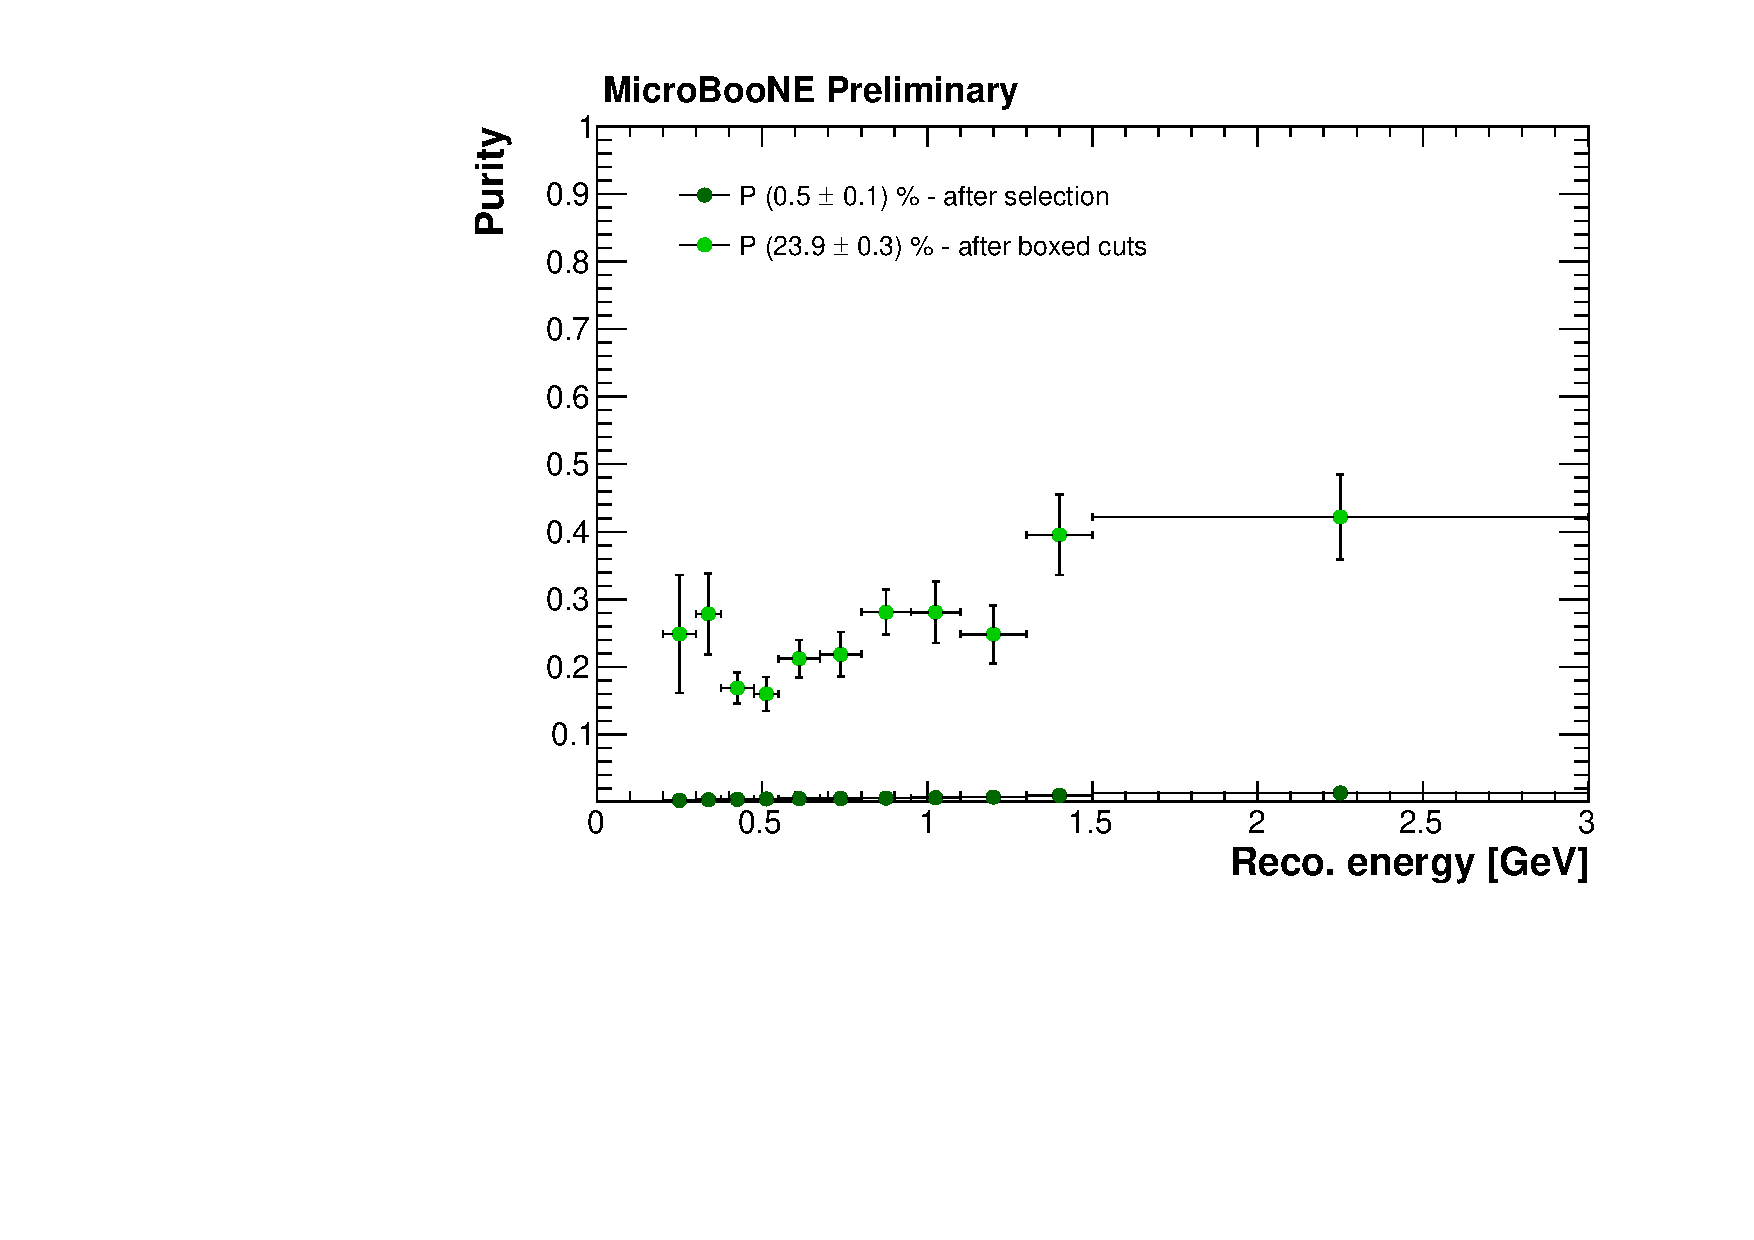
\includegraphics[width=\linewidth]{figures/purity_after.pdf}
    \caption{Purity} 
  \end{subfigure}
  \caption{Left: $\nu_{e}$ CC$0\pi$-Np reconstruction efficiency as a function of the true $\nu_{e}$ energy before and after the background-rejection cuts. Right: $\nu_{e}$ CC$0\pi$-Np purity as a function of the reconstructed energy before and after the background-rejection cuts.}
  \label{fig:effafter}
\end{figure}